%!TEX program = xelatex

\documentclass[a4paper, openany, oneside]{memoir}
\usepackage[no-math]{fontspec}
\usepackage{pgfplots}
\usepackage{float}
\pgfplotsset{compat=newest}
\usepackage{commath}
\usepackage{mathtools}
\usepackage{amssymb}
\usepackage{amsthm}
\usepackage{booktabs}
\usepackage{todonotes}
\usepackage{mathtools}
\usepackage{xcolor}
\usepackage[separate-uncertainty=true, per-mode=symbol]{siunitx}
\usepackage{listings}
\usepackage[american inductor, european resistor]{circuitikz}
\usepackage{amsmath}
\usepackage{amsfonts}
\usepackage{ifxetex}
\usepackage[dutch,english]{babel}
\usepackage[backend=bibtexu,texencoding=utf8,bibencoding=utf8,style=ieee,sortlocale=en_GB,language=auto]{biblatex}
\usepackage[strict,autostyle]{csquotes}
\usepackage{import}
\usepackage{standalone}
\usepackage{bookmark,hyperref}
\usepackage{xcolor,mdframed}
\usepackage{tikz}
\usepackage{framed}
\usepackage{float}
\usepackage{tabularx}
\usepackage{graphicx,adjustbox}
\usepackage{rotating}
\usepackage{pdfpages}
\usepackage{enumitem}
\usepackage{calc}
\usepackage{pgfplots}
\usepackage{filecontents}
\usepackage{caption}
\usepackage{subcaption}
\usepackage{lettrine}

\newcolumntype{Y}{>{\raggedright\arraybackslash}X} % Left-justified text in tabularx environment

\ifxetex{} % Fonts laden in het geval dat je met Xetex compiled
    \usepackage{fontspec}
    \defaultfontfeatures{Scale=MatchLowercase, Ligatures=TeX} % To support LaTeX quoting style
    %\setromanfont{Palatino Linotype} % Tover ergens in Font mapje in root.
    \setsansfont{Avenir Next LT Pro}
    \setromanfont{Adobe Caslon Pro} % Tover ergens in Font mapje in root.
    \setmonofont{Source Code Pro}
\else % Terug val in standaard pdflatex tool chain. Geen ondersteuning voor OTT fonts
    \usepackage[T1]{fontenc}
    \usepackage[utf8]{inputenc}
\fi
\usepackage[noabbrev, capitalize]{cleveref}
\usepackage{ifthen}
\usepackage{titlesec}
\usepackage{titlecaps}

\newcommand{\references}[1]{\begin{flushright}{#1}\end{flushright}}
\renewcommand{\vec}[1]{\boldsymbol{\mathbf{#1}}}
\newcommand{\uvec}[1]{\boldsymbol{\hat{\vec{#1}}}}
\newcommand{\mat}[1]{\boldsymbol{\mathbf{#1}}}
\newcommand{\fasor}[1]{\boldsymbol{\tilde{\vec{#1}}}}
\newcommand{\cmplx}[0]{\mathrm{j}}
\renewcommand{\Re}[0]{\operatorname{Re}}
\newcommand{\Cov}{\operatorname{Cov}}
\newcommand{\Var}{\operatorname{Var}}
\newcommand{\proj}{\operatorname{proj}}
\newcommand{\Perp}{\operatorname{perp}}
\newcommand{\col}{\operatorname{col}}
\newcommand{\rect}{\operatorname{rect}}
\newcommand{\sinc}{\operatorname{sinc}}
\newcommand{\lcm}{\operatorname{lcm}}
%\newcommand{\gcd}{\operatorname{gcd}}
\newcommand{\F}{\mathcal{F}}
\newcommand{\DTFT}{\mathcal{F}_*}
\newcommand{\conj}[1]{#1^*}
\renewcommand{\mod}{\operatorname{mod}}
\newcommand{\rot}{\operatorname{rot}}
\newcommand{\vecsc}[1]{\vec{\textsc{\textbf{#1}}}}
\renewcommand{\ss}[1]{_{#1}}

% Label without linebreak breaker
\newcommand{\lab}[1]{\label{#1}\nolinebreak}

\newtheorem{definition}{Definition}
\newtheorem{theorem}{Theorem}


\DeclareSIUnit{\voltampere}{VA} %apparent power
\DeclareSIUnit{\pii}{\ensuremath{\pi}}

\hypersetup{%setup hyperlinks
    colorlinks,
    citecolor=black,
    filecolor=black,
    linkcolor=black,
    urlcolor=black
}

% Example boxes
\usepackage{fancybox}
\usepackage{framed}
\usepackage{adjustbox}
\newenvironment{simpages}%
{\AtBeginEnvironment{itemize}{\parskip=0pt\parsep=0pt\partopsep=0pt}
\def\FrameCommand{\fboxsep=.5\FrameSep\shadowbox}\MakeFramed{\FrameRestore}}%
{\endMakeFramed}

% Impulse train
\DeclareFontFamily{U}{wncy}{}
\DeclareFontShape{U}{wncy}{m}{n}{<->wncyr10}{}
\DeclareSymbolFont{mcy}{U}{wncy}{m}{n}
\DeclareMathSymbol{\Sha}{\mathord}{mcy}{"58}

\setlength{\parindent}{0pt}
\nonzeroparskip

% Block environment configuration
\newcommand{\BlockLeftMargin}{20pt}
\newcommand{\BlockLeftMarginText}{25pt}
\newcommand{\BlockLeftMarginTextSpacing}{10pt}

% Own colours
\definecolor{gray75}{gray}{0.75}

% Block environment
\newenvironment{block}[3]{%
\makebox{\hspace{-\spinemargin}%
\begin{tikzpicture}[overlay]
    \draw [thick,color=gray75] (\BlockLeftMargin, 0) -- (\paperwidth - \spinemargin, 0);
    \node at (\BlockLeftMarginText, -0.9) [align=left, text width=\spinemargin - \BlockLeftMarginText - \BlockLeftMarginTextSpacing, anchor=west, text depth=1cm] {\textbf{\textsc{#1}}\newline\textit{#3}};
\end{tikzpicture}}%
\nopagebreak\\[0.25em]\ifthenelse{\equal{#2}{}}{}{(\textit{#2}.) }\nopagebreak\nolinebreak}
{\nopagebreak\\[-0.25em]%
\makebox{\hspace{-\spinemargin}%
\begin{tikzpicture}[overlay, remember picture]
    \draw [thick,color=gray75] (\spinemargin,0) -- (\paperwidth - \spinemargin,0);
\end{tikzpicture}} \vspace{0.5em}}

% Theorem
\newcounter{blockTheoremCounter}
\crefname{blockTheoremCounter}{Theorem}{Theorems}
\Crefname{blockTheoremCounter}{Theorem}{Theorems}

\newenvironment{blockTheorem}[1][]{%
\refstepcounter{blockTheoremCounter}%
\begin{block}{theorem \theblockTheoremCounter}{#1}{}}
{\end{block}}

% Definition
\newcounter{blockDefinitionCounter}
\crefname{blockDefinitionCounter}{Definition}{Definitions}
\Crefname{blockDefinitionCounter}{Definition}{Definitions}

\newenvironment{blockDefinition}[1][]{%
\refstepcounter{blockDefinitionCounter}%
\begin{block}{definition \theblockDefinitionCounter}{#1}{}}
{\end{block}}

% Proof
\newcounter{blockProofTheoremCounter}
\crefname{blockProofTheoremCounter}{Proof}{Proofs}
\Crefname{blockProofTheoremCounter}{Proof}{Proofs}

\newenvironment{blockProofTheorem}[1]{%
\refstepcounter{blockProofTheoremCounter}%
\begin{block}{proof of \\ theorem #1}{}{}}
{\qed\end{block}}

% Detail
\newcounter{blockDetailCounter}
\crefname{blockDetailCounter}{Detail}{Details}
\Crefname{blockDetailCounter}{Detail}{Details}

\newenvironment{blockDetail}[1][]{%
\refstepcounter{blockDetailCounter}%
\begin{block}{detail \theblockDetailCounter}{#1}{}}
{\end{block}}

% Redesign chapter headings
\newcommand{\chapternumber}{\thechapter}
\newcommand{\hsp}{\hspace{20pt}}
\titleformat{\chapter}[hang]{\Huge\bfseries}{\chapternumber\hsp\textcolor{gray75}{|}\hsp}{0pt}{\Huge\bfseries}

% Remove headers
% \addtopsmarks{headings}{}{
%   \createmark{chapter}{left}{nonumber}{}{}
% }
% \pagestyle{headings} % Activate changes

% Capitalise headers in a regular way
\renewcommand*{\memUChead}[1]{\titlecap{#1}}

% \hfill for math mode
\newcommand{\pushright}[1]{\intertext{\hfill$\displaystyle #1$}}
\newcommand{\pushline}{\hskip \textwidth minus \textwidth}
\newcommand{\matlab}{\textsc{Matlab}}

\definecolor{code-grey}{HTML}{DDDDDD}
\newcommand{\lib}[1]{\textsf{#1}}
\newcommand{\file}[1]{\textsf{#1}}
\newcommand{\func}[1]{\colorbox{code-grey}{\texttt{#1}}}
\newcommand{\class}[1]{\colorbox{code-grey}{\texttt{#1}}}

% Setup actiepunten
\newenvironment{important}[1][]{%
   \begin{mdframed}[%
      backgroundcolor={red!15}, hidealllines=true,
      skipabove=0.7\baselineskip, skipbelow=0.7\baselineskip,
      splitbottomskip=2pt, splittopskip=4pt, #1]%
   \makebox[0pt]{% ignore the withd of !
      \smash{% ignor the height of !
         \fontsize{32pt}{32pt}\selectfont% make the ! bigger
         \hspace*{-19pt}% move ! to the left
         \raisebox{-2pt}{% move ! up a little
            {\color{red!70!black}\sffamily\bfseries !}% type the bold red !
         }%
      }%
   }%
}{\end{mdframed}}
\newcommand{\excl}[1]{
\begin{important}
  \textbf{#1}
\end{important}
}

\makeatletter
\newcommand\footnoteref[1]{\protected@xdef\@thefnmark{\ref{#1}}\@footnotemark}
\makeatother

% Allow page breaks in display environments
%\allowdisplaybreaks
% S unit for use in Mega Samples per second
\DeclareSIUnit\sample{S}

\newcommand{\CC}{C\nolinebreak\hspace{-.05em}\raisebox{.3ex}{ \textbf{+}}\nolinebreak\hspace{-.10em}\raisebox{.3ex}{\textbf{+}}}
\def\CC{{C\nolinebreak[4]\hspace{-.05em}\raisebox{.3ex}{\textbf{++}}}}


\newcommand{\partauthor}[1]{\gdef\@partauthor{#1}}
\renewcommand{\printparttitle}[1]{
  \parttitlefont #1\\
  \vspace{1.5cm}
  \textnormal{\Large \@partauthor}
}
\addbibresource{../../../../includes/bibliography.bib}

\begin{document}
\section{Preliminaries}

Vectors are denoted by lower-case bold-faced letters and matrices are denoted by upper-case bold-faced letters. Unless stated otherwise, a vector is always assumed to be a column vector. The complex conjugate of a vector $\vec{x}$ is denoted by $\bar{\vec{x}}$. The inner product of an inner product space is denoted by $\cdot$. We now introduce notation to denote elements of vectors and matrices.

\begin{blockDefinition}[Vector Element]
    Let $\vec{x} \in \mathbb{C}^N$. Then $(\vec{x})_i$ denotes the $i$'th element of $\vec{x}$ for $i = 1,\ldots,N$.
\end{blockDefinition}

\begin{blockDefinition}[Matrix Element]
    Let $\mat{A}$ be an $M \times N$ matrix. Then $(\mat{A})_{i,j}$ denotes the $j$'th element of the $i$'th row of $\mat{A}$ for $i = 1,\ldots,M$ and $j=1,\ldots,N$.
\end{blockDefinition}

We will need notation to denote two uncommon vector operations.

\begin{blockDefinition}[Subvector]
    Let $\vec{x} \in \mathbb{C}^N$. Then $\vec{x}[a,b]$ denotes a vector $\vec{z} \in \mathbb{C}^{b-a+1}$ such that $(\vec{z})_i = (\vec{x})_{i+a-1}$ for $i = 1,\ldots,b-a+1$.
\end{blockDefinition}

Note that a subvector includes both boundary elements.

\begin{blockDefinition}[Submatrix]
    Let $\mat{A}$ be an $M \times N$ matrix. Then $\mat{A}[a,b]$ denotes the $M \times b-a+1$ matrix consisting of columns $a,\ldots,b$ of $\mat{A}$.
\end{blockDefinition}

Also a submatrix includes both boundary elements.

\begin{blockDefinition}[Reverse of Vector]
    Let $\vec{x} \in \mathbb{C}^N$. Then the reverse of $\vec{x}$ denotes a vector $\vec{y} \in \mathbb{C}^N$ such that $(\vec{y})_i = (\vec{x})_{N-i+1}$ for $i = 1,\ldots,N$.
\end{blockDefinition}

We now define the convolution operator as a closed binary operation on vectors. The definition is similar to the definition of convolution for discrete signals. This implies that results similar to well-known theorems can be obtained.

\begin{blockDefinition}[Convolution]
    Let $\vec{x} \in \mathbb{C}^N$ and $\vec{y} \in \mathbb{C}^M$. Then $\vec{x} \ast \vec{y}$ denotes a vector $\vec{z} \in \mathbb{C}^{N+M-1}$ such that
    \begin{align*}
        (\vec{z})_i = \sum_{k=1}^{N} (\vec{x})_k (\vec{y})_{i-k+1}
    \end{align*}
    where $(\vec{x})_i=0$ for $i < 1$ and $i > N$ and $(\vec{y})_i=0$ for $i < 1$ and $i > M$.
\end{blockDefinition}

\begin{blockTheorem}[Commutativity of Convolution] \label{th:conv-comm}
    Let $\vec{x} \in \mathbb{C}^N$ and $\vec{y} \in \mathbb{C}^M$. Then $\vec{x} \ast \vec{y} = \vec{y} \ast \vec{x}$.
\end{blockTheorem}

The proof of \cref{th:conv-comm} will be given in \cref{sec:proofs}. We also define correlation as a closed binary operation on vectors. The definition is again similar to the definition of correlation for discrete signals.

\begin{blockDefinition}[Deterministic Cross-correlation]
    Let $\vec{x} \in \mathbb{C}^N$ and $\vec{y} \in \mathbb{C}^M$. Then $\vec{x} \circ \vec{y}$ denotes a vector $\vec{z} \in \mathbb{C}^{N+M-1}$ such that
    \begin{align*}
        (\vec{z})_i = \sum_{k=1}^{N} (\vec{x})_k (\conj{\vec{y}})_{M-i+k}
    \end{align*}
    where $(\vec{x})_i=0$ for $i < 1$ and $i > N$ and $(\vec{y})_i=0$ for $i < 1$ and $i > M$.
\end{blockDefinition}

Furthermore, we define the Hadamard product as a closed binary operation on vector.

\begin{blockDefinition}[Hadamard Product]
    Let $\vec{x} \in \mathbb{C}^N$ and $\vec{y} \in \mathbb{C}^N$. Then $\vec{x} \odot \vec{y}$ denotes a vector $\vec{z} \in \mathbb{C}^N$ such that $(\vec{z})_i = (\vec{x})_i (\vec{y})_i$ for $i = 1,\ldots,N$.
\end{blockDefinition}

Note that $\odot$ is similar to $\cdot$, since the inner product and Hadamard product are closely related.
The following theorem identifies the expected value of the correlation operator.

\begin{blockTheorem} \lab{th:corr-unbiased}
    Let $X[n]$ and $Y[n]$ be wide sense stationary stochastic processes. Let $\vec{x} \in \mathbb{C}^N$ and $\vec{y} \in \mathbb{C}^M$ be such that $(\vec{x})_i = X[i]$ for $i=1,\ldots,N$ and $(\vec{y})_i = Y[i]$ for $i=1,\ldots,M$. Furthermore, let $r[n]$ be a discrete signal such that $r[i] = (\vec{x} \circ \vec{y})_{i+M}$ for $i = -M+1,\ldots,N-1$. Then $r[i]$ is an unbiased estimator of $W[i]R_{X,Y}[i]$ where
    \begin{align*}
        W[i] = \begin{cases}
            i + M & \text{if } -M + 1 \le i \le -M + K, \\
            K & \text{if } -M + K < i < N - K, \\
            N - i & \text{if } N - K \le i \le N - 1, \\
            0 & \text{elsewhere,}
        \end{cases}
    \end{align*}
    where $K = \min\{N,M\}$.
\end{blockTheorem}

Finally, we extend the use of dots to denote finite sequences.

\begin{blockDefinition} \lab{def:dots-extended}
    Let $N \in \mathbb{N}$ and let $S=\{(a,b) \in \mathbb{N} \times \mathbb{N} : a < b \le N\}\cup \{(1,1)\}$. Then $(1,1),\ldots,(N,N)$ denotes the sequence of all elements in $S$ such that $(1,1)$ is first and $(a,b) \in S$ comes before $(c,d) \in S$ when $a < c$, or when $b < d$ if $a = c$.
\end{blockDefinition}

Note that $(1,1),\ldots,(N,N)$ represents in an $N \times N$ grid a corner point and the dots below the diagonal. This is pictured in \cref{fig:dots-extended}.

\begin{figure}[H]
    \centering
    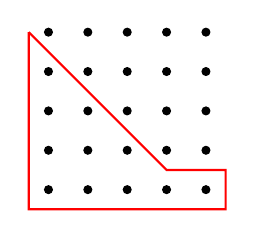
\begin{tikzpicture}
        \draw [black, fill=black] (0,0) circle [radius=0.05];
        \draw [black, fill=black] (0,0.5) circle [radius=0.05];
        \draw [black, fill=black] (0,1) circle [radius=0.05];
        \draw [black, fill=black] (0,1.5) circle [radius=0.05];
        \draw [black, fill=black] (0,2) circle [radius=0.05];

        \draw [black, fill=black] (0.5,0) circle [radius=0.05];
        \draw [black, fill=black] (0.5,0.5) circle [radius=0.05];
        \draw [black, fill=black] (0.5,1) circle [radius=0.05];
        \draw [black, fill=black] (0.5,1.5) circle [radius=0.05];
        \draw [black, fill=black] (0.5,2) circle [radius=0.05];

        \draw [black, fill=black] (1,0) circle [radius=0.05];
        \draw [black, fill=black] (1,0.5) circle [radius=0.05];
        \draw [black, fill=black] (1,1) circle [radius=0.05];
        \draw [black, fill=black] (1,1.5) circle [radius=0.05];
        \draw [black, fill=black] (1,2) circle [radius=0.05];

        \draw [black, fill=black] (1.5,0) circle [radius=0.05];
        \draw [black, fill=black] (1.5,0.5) circle [radius=0.05];
        \draw [black, fill=black] (1.5,1) circle [radius=0.05];
        \draw [black, fill=black] (1.5,1.5) circle [radius=0.05];
        \draw [black, fill=black] (1.5,2) circle [radius=0.05];

        \draw [black, fill=black] (2,0) circle [radius=0.05];
        \draw [black, fill=black] (2,0.5) circle [radius=0.05];
        \draw [black, fill=black] (2,1) circle [radius=0.05];
        \draw [black, fill=black] (2,1.5) circle [radius=0.05];
        \draw [black, fill=black] (2,2) circle [radius=0.05];

        \draw [red, thick] (-.25, 2) -- (-0.25, -0.25) -- (2.25, -0.25) -- (2.25, 0.25) -- (1.5, 0.25) -- (-.25, 2);
    \end{tikzpicture}
    \caption{Visualisation of $(1,1),\ldots,(N,N)$}
    \label{fig:dots-extended}
\end{figure}


\begin{blockTheorem} \lab{th:dots-extended}
    Let $N \in \mathbb{N}$. Then $(1,1),\ldots,(N,N)$ is finite and has length $\frac{1}{2}N(N-1)+1$.
\end{blockTheorem}

\end{document}